\section{Background \& Motivation}
\label{sec:bg}
%\subsection{Functions as a Service}
%\label{sec:bg:faas}

Functions as a Service (FaaS) allows users to register small snippets of function code that get executed in response to some event or trigger (such as an HTTP request, message queue event, etc.)
~\cite{serverless-cacm-21, aws-lambda, google-functions,azure-functions}. 
These functions must be stateless: a new execution environment may be created for every invocation (and can be destroyed after the function returns). 
The function code also contains all the necessary code and data dependencies (such as imported libraries and packages), and thus functions may spend significant time being \emph{initialized} before the event-handling code can execute. 
Functions are executed inside virtual execution environments such as hardware virtual machines, OS containers like Docker, or even language-based runtimes such as javascript WASM~\cite{shillaker2020faasm}.
Function initialization, i.e., creating the execution environment and resolving code/data dependencies, can take 100s of milliseconds, and this ``cold start'' can significantly increase the latency of small functions~\cite{du2020catalyzer, faascache-asplos21}.
Initialized function sandboxes can be retained in memory, and this \emph{keep-alive} provides faster ``warm-starts''~\cite{faascache-asplos21}. 
%
Since functions are arbitrary user-code, they are extremely heterogeneous in their execution characteristics and resource requirements. 
% For instance, the FaaS workload traces provided by Azure shows that the workload is buextremely bursty and heavy-tailed across many dimensions: a small fraction of functions are responsible for a majority of invocations, and some large functions contribute to a majority of the resource consumption.
For instance, the Azure FaaS trace~\cite{shahrad_serverless_2020} shows that the 50th and 95th percentile of execution time can range from 1 second to 1 minute; and the inter-arrival-time from 1 second to 15 minutes respectively.

% \vspace*{-8pt}
\subsection{FaaS Control Planes}
\label{sec:bg:cplane}

All aspects of function execution are orchestrated by a FaaS \emph{control plane}, which are implemented by frameworks like OpenWhisk~\cite{openwhisk}.
For using a FaaS service, the user interacts with the control plane for registering and invoking functions, tracking their status, etc.
The control plane manages the resources of a cluster of servers, and schedules functions on to them based on its load-balancing policies.

%FaaS is a relatively new workload paradigm, and control planes are still evolving and maturing.
%OpenWhisk is a popular framework which has been used as a platform for investigating and optimizing many facets of FaaS execution.

In OpenWhisk, user requests for invoking a function go through a reverse proxy (NGINX) to the central \emph{controller}, which implements, among other things, load-balancing (a variant of consistent hashing with bounded loads by default).
The controller puts the function invocation request into a shared Apache Kafka~\cite{kafka} queue.
Inside the worker, the invoker service pulls function invocations from the Kafka queue based on that worker's own resource availability.
Docker containers running a Go-based control plane agent are used to isolate functions, and each worker maintains a container pool of initialized/warm containers.
% A worker ultimately runs the function, and the control plane extends across the worker as well. 
%OpenWhisk strives to provide exactly-once semantics (although this hasn't been tested or verified) by logging function results in CouchDB. Kafka and CouchDB in the critical path. 
OpenWhisk logs function results in a CouchDB instance.
Importantly, both Kafka and CouchDB are on the critical path, and add 100s of ms to invocation latency.
%
OpenWhisk is highly modular and distributed, with many networked services.
All of these, combined with the JVM GC (it is implemented in Scala), results in large and unpredictable latency spikes~\cite{faaslb-hpdc22, hotcarbon22-faas}, with slowdowns of more than $10,000\times$ reported~\cite{zuk_call_2022}. 
%For instance, Stretch factors shown in~\cite{zuk} of 10,000, indicating that the overhead is 10,000 more than the actual processing latency, and with response times of 100s of seconds. 

\begin{comment}
Shared kafka queue for scheduling and assignment of invocations.
Contended.
Ours simpler design: locality enforced through multiple independent loosely coupled components: CH-BL load balancer, and queuing at the invoker for tolerating bursts. 

The burst mitigation is done again using many techniques.
Increase queue size, overcommit resources and increase concurrency, forward, and finally elastic scaling.

OS level preemption is useful, since function invocation is not confined to a single process but many components such as containerization layer. The resource usage is also not uniform, but bursty and low average.

Stretch factors shown in~\cite{zuk} of 10,000, indicating that the overhead is 10,000 more than the actual processing latency, and with response times of 100s of seconds. 

\noindent \textbf{Control planes}  (such as OpenWhisk~\cite{openwhisk})  handle all aspects of function execution. 
This control plane manages a cluster of servers to run functions on, and implements function scheduling, load-balancing, resource monitoring, function status tracking, storing function results, logging, etc. 
It is also responsible for performance optimizations for functions such as keep-alive~\cite{faascache-asplos21} to mitigate function cold start overheads due to the sandboxing and function initialization overheads. 
%\emph{Paint a picture of what all it does.}
The control plane itself is highly distributed with many components such as API gateways, distributed message queues (such as Kafka), and databases. % (like CouchDB).
Even on a single server, a function's execution is orchestrated through many components, as shown in Figure~\ref{fig:faasmeter-iluvatar}. 
\end{comment}

% \vspace*{-8pt}
\subsection{Why a new FaaS control plane?}
\label{sec:bg:ynew}

% Why did we embark on this mission in the first place?

We believe that the FaaS control plane is an important component of the modern cloud ecosystem, and presents many optimization opportunities and interesting research questions in system design. 

\begin{figure}
  \centering  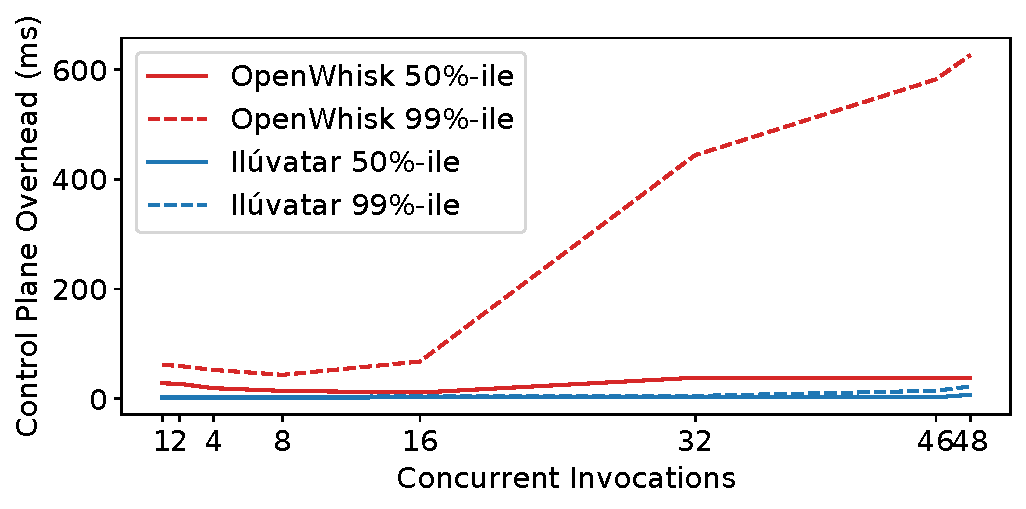
\includegraphics[width=0.4\textwidth]{iluvatar/graphs/scaling/pyaes/overhead-scaling.pdf}
  % \vspace*{-6pt}
  \caption{The latency overhead of the control plane, as the number of concurrent invocations increases. OpenWhisk overhead is significant and has high variance, resulting in high tail latency. \sysname~reduces this overhead by 100x. }
  \label{fig:ow-scaling}
    % \vspace*{-6pt}
\end{figure}


\noindent \textbf{Performance.}
%
Because of its central role in coordinating all aspects of function execution, the control plane plays a major role in determining function performance. 
Managing the function execution lifecycle for hundreds of concurrent invocations imposes a \emph{control plane overhead}, and increases the end-to-end latency.
This control plane overhead can be significant, and affects \emph{all} function invocations, including and especially the ``warm starts''. 
%Time spent in the control plane is simply measured by subtracting the execution time of the function code from the overall end-to-end latency.
This overhead (end-to-end latency minus the function code execution time) for the PyAES function from FunctionBench~\cite{kim2019functionbench} is shown in Figure~\ref{fig:ow-scaling}. 

The figure shows the 50 and 99 percentile overheads as the number of concurrent invocations are increased.
In each case, we are invoking the function repeatedly in a closed-loop, and concurrent invocations are achieved by using multiple client threads.
All invocations are warm starts.
The experiment is run on a 48 core server (more details in Section~\ref{sec:eval}), and the figure thus shows the performance at low and medium load conditions. 

From Figure~\ref{fig:ow-scaling}, we can see that the OpenWhisk latency overhead is more than 10ms,  which is already a significant increase in latency for small functions which dominate real-world FaaS workloads.
Worryingly, the 99 percentile overhead is much higher, and rises to as much as 600ms.
We also see strange inversions in the scaling behavior: the overhead reduces for certain load-levels, and then increases again.
This high overhead, high variance, and uncertain scaling behavior, results in many challenges for FaaS \emph{providers}. 
Due to these issues, low-latency functions see severe performance degradation, and resource provisioning and capacity planning becomes harder due to the high variance and performance unpredictability. 
%

Some of these latency overheads are an artifact of the architecture. 
The shared Kafka function queue can be a major bottleneck; and there are no explicit backpressure or load regulation mechanisms, which is compounded by the CPU overcommitment. 
%
For the sake of comparison, the figure also shows the latency overhead of \sysname~in the same environment. 
We are able to achieve a per-invocation mean overhead of less than 2ms for almost all the load conditions.
Importantly, the tail overhead is also small: less than 3ms for less than 32 concurrent invocations, rising to 10ms when the system is saturated.


To emphasize, for a median function in the Azure workload which runs for 500 ms, OpenWhisk can increase its latency by 100\%.  
Thus, the control plane plays a crucial role in function performance.
We note that these are the best-case warm-start latencies, when the function's containers is fully initialized and in memory. 
Since function cold starts impose such a major performance penalty (increasing latency by more than $10\times$), mitigating them has been a major research focus. 
However, because of temporal and spatial locality of access, caching and prefetching techniques can be extremely effective, and the cold start rate is often less than $1\% $ of all invocations~\cite{faascache-asplos21}. 
The majority of invocations are thus ``warm'', where the performance is dominated by control plane overheads.
%\emph{We thus need a low-latency, low-jitter control plane.}

\noindent \textbf{System Design.}
%
As evidenced by the OpenWhisk architecture presented earlier, FaaS control planes are large, complex distributed systems.
Due to the continually evolving needs of FaaS applications and emergence of new sandboxing techniques (such as lightweight VMs like Firecracker~\cite{firecracker-nsdi20}), they are sandwiched between the scale and heterogeneity of FaaS workloads on one hand, and the deep stack of OS and virtualization components on the other. 

For instance, systems for running web services or microservices do not have to deal with large and highly variable sandbox management overheads, nor with highly heterogeneous request sizes.
For reducing tail latency, these systems can often rely on the OS CPU scheduler for processor sharing, can do CPU allocation at very fine granularity~\cite{kaffes2019shinjuku}, use queuing theory techniques~\cite{prekas2017zygos}, etc. 
At the other extreme, for longer running containers and VMs, their control planes, like OpenStack or Kubernetes face a much lower rate of VM arrivals and departures. and can do careful and ``hard'' resource allocation using bin-packing~\cite{cortez2017resource}.


Functions are highly heterogeneous, and can be seen as both latency-sensitive web requests \emph{and} large containers requiring significant system resources for several seconds. 
FaaS control planes thus have to do \emph{both} low-latency allocation \emph{and} pack CPU and memory resources on their servers carefully to maintain high system utilization.
%
%We posit that these competing needs present new challenges in large-scale distributed resource allocation.
Thus FaaS control planes are one of the more perfect microcosms of challenges in resource management and control in large scale distributed computing. 

A clean-slate control plane design helps us investigate the fundamental performance tradeoffs and challenges in this fast-evolving ecosystem.
Our new implementation also helps to identify the current performance bottlenecks and new avenues of OS optimizations. 


\noindent \textbf{Platform for Experimental Systems Research.}
%
Performance-focused FaaS research is already challenging due to the extreme scale and heterogeneity of the workloads.
These challenges are compounded by existing control planes like OpenWhisk that are unfortunately highly unpredictable.
The control plane jitter and the extreme bimodal cold vs. warm latencies makes it difficult to do reliable and reproducible research~\cite{mytkowicz2009producing}, and subtle environmental and configuration effects can mask the true effects of new research optimizations.
However, it continues to be a key component in developing and evaluating FaaS research~\cite{akkus_sand_2018, shahrad_serverless_2020, faascache-asplos21, faaslb-hpdc22, zhou2022aquatope, ensure-faas-acsos20, alzayat_groundhog_2022}. 
%OpenWhisk is a popular framework which has been used as a platform for investigating and optimizing many facets of FaaS execution.
With OpenWhisk, function performance can be severely affected by a myriad of configuration options, such as insufficient memory for CouchDB, networking configuration, Docker configuration, etc. 

Given the importance of the control plane, we want \emph{predictable} performance to a large degree. 
In our experience, research in FaaS is often hindered by the large overheads and complexity of existing control planes. 
Thus, \sysname~is designed from the ground-up to be lightweight and provide predictable performance under different conditions. 
Our system implementation can potentially accelerate the development of new optimizations, clarify  our understanding of performance characteristics of this relatively new stack, and provide a platform for robust experiments. 
% Establishing a shared open platform enables easy comparison between research work
With a robust platform, the community can share knowledge and advances, while being able to compare against a well-known and trusted baseline.

\begin{comment}
\textbf{Why write from scratch instead of improving existing ones?}

A clean-slate design also gives us the opportunity for understanding the design tradeoffs that could be helpful for general FaaS research and 

Lightweight/minimal ones like faasd exist. But again, written in go, not performance focused, and implementing all the desired research features would make it a different.

We also wanted this to be a design exercise in exploring the tradeoff between being lightweight and high performance vs. being extensible and ``full-featured''.
\end{comment}


%%% Local Variables:
%%% mode: latex
%%% TeX-master: "paper"
%%% End:
